\section{Fit to ADC Output}
\label{Sec:fitToADCOutput}
Although in general a 3-strip pixel can be odd shaped, a 2-strip pixel can be straightforward. 
This two layer correlation creates trapezoidal bins formed by the overlap of two different strip 
orientations\footnote{All of the studies in this section were primarily focused on the u strip attenuations, 
rather than the v/w strips.}. An example of one of these trapezoids outlined in black can be seen in Fig.~\ref{fig:stripwidth}. 
Each one of these trapezoids should have a ADC readout value. The width of this physical bin can be found by

\begin{equation}
    s = \frac{w}{\sin{\alpha}}
    \label{eq:s}
\end{equation}
or
\begin{equation}
    s = \frac{w}{\cos{\beta}},
\end{equation}
where $w$ is a single scintillator strip width ($\approx 4.5$cm).
Statistically one might expect some sort of peak describing the distribution of values. The centroid of this 
distribution is used as a data point at that center of that physical bin.

\begin{figure}[h]
\centering
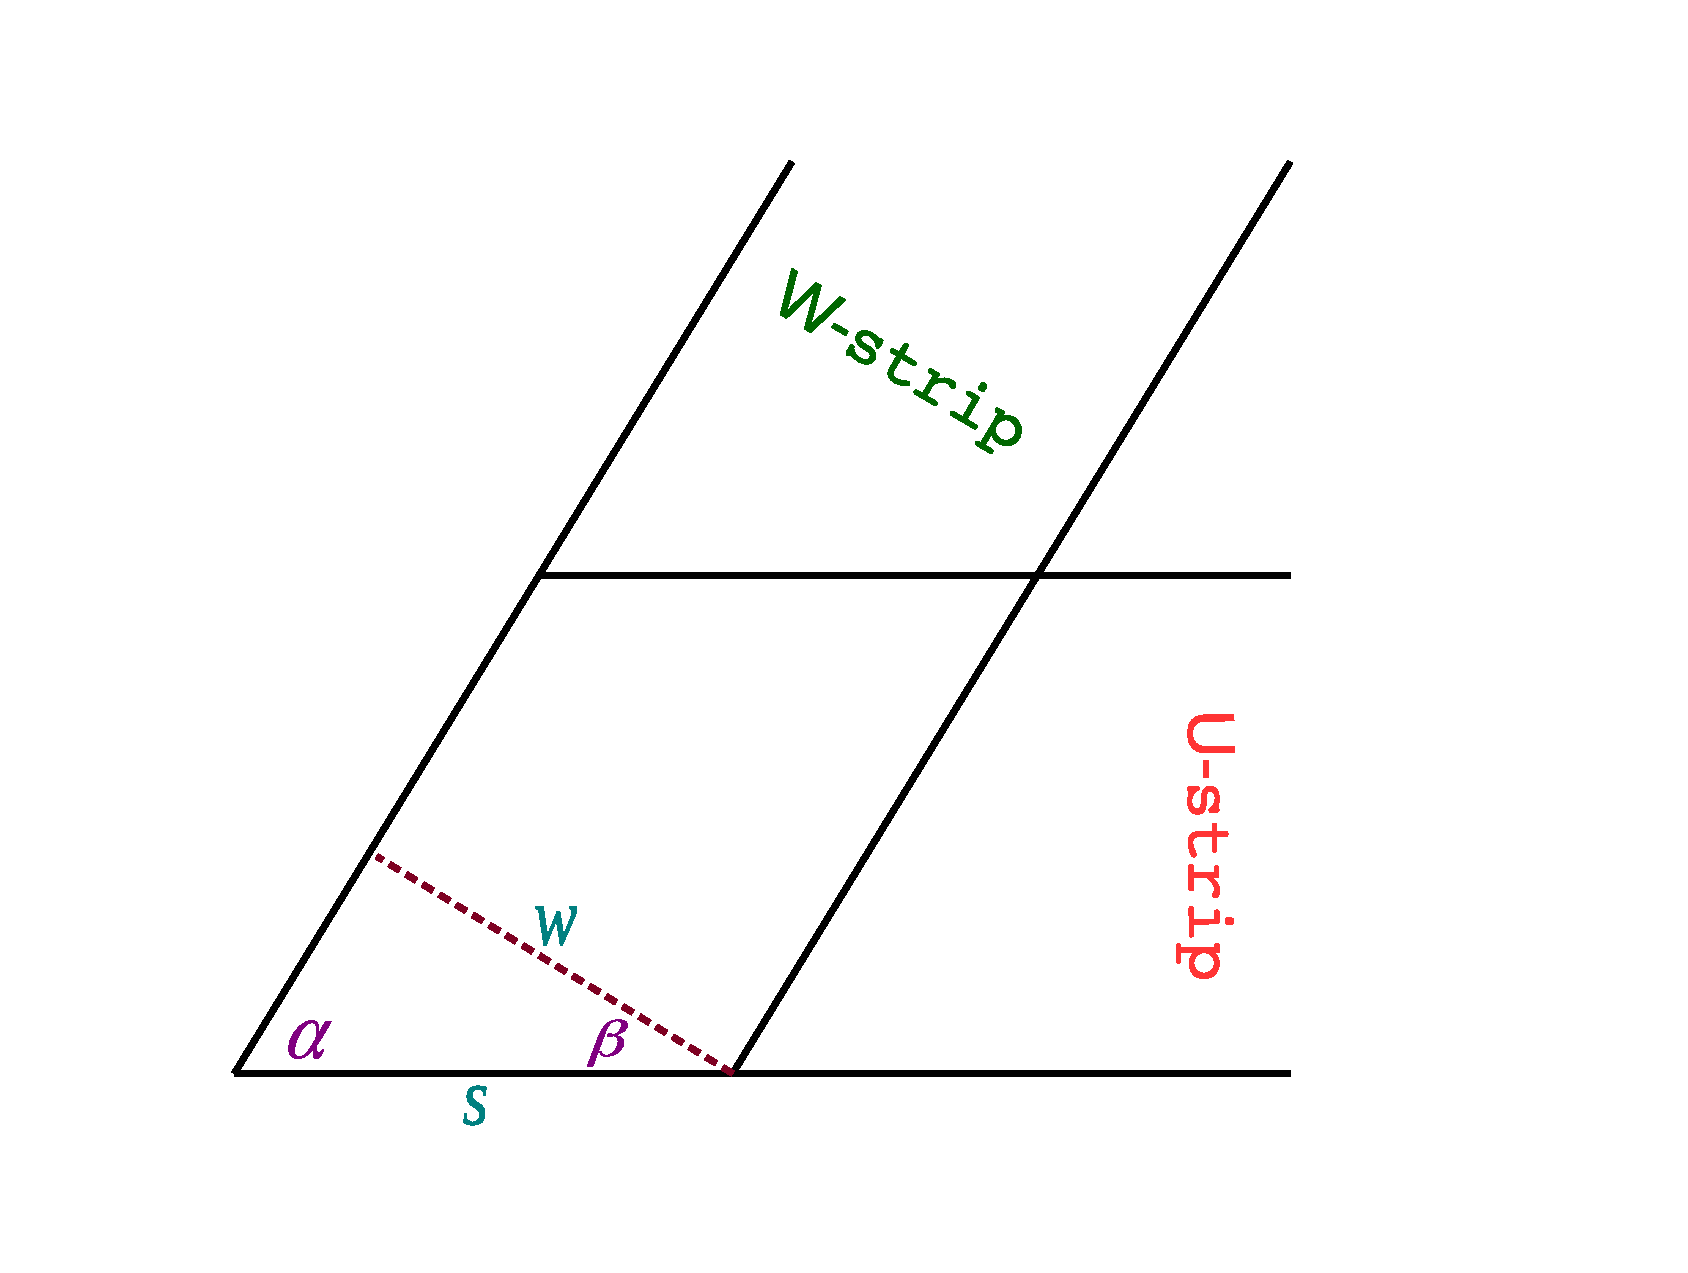
\includegraphics[width= 3in, keepaspectratio = true]{trapezoidUWintersection}%stripwidth
\caption{Shown is an outline of a generic intersection of a u and w strip. The distance between the trapezoidal
 area and the PCAL edge can be represented by a linear function of $s$.}
\label{fig:stripwidth}
\end{figure}

\FloatBarrier
\subsection{Signal Shape}
The desired outcome is to approximate the signal by a simple function, for instance a Gaussian function.
Upon investigation the integrated ADC values appear to be a combination of a Gaussian and exponential fits.

\begin{figure}[h]
    \centering
    \includegraphics[width= 4in, keepaspectratio = true]{distribution}
    \caption{Shown is an example of the distribution of the ADC readout from one u/w trapezoidal bin 
    (specifically the logical numbers u =67, w=50). The red line is a fit to an exponential combined with 
    a Gaussian distribution.}
    \label{fig:distribution}
\end{figure}

This type of background can be seen for every physical two layered bin along any strip.

\begin{figure}[h]
    \centering
    \includegraphics[width= 6in, keepaspectratio = true]{allstrip67}
    \caption{Shown is an example of all the distributions of the ADC readout from the 67th logical u strip.}
    \label{fig:allstrip67}
\end{figure}


\FloatBarrier
\subsubsection{Fit function}
Upon initial inspection the distribution is fit to an exponential and a Gaussian. 
The exponential is background/noise in most cases, whereas the Gaussian represents near perpendicular cosmic ray hits. 
The centroid of the Gaussian is extracted and determined to be the primary light intensity in that trapezoidal bin.

This plan works well for most interior physical bins. However, after looking at the strips corresponding to 
the edges of the PCAL unit, it is realized this can't be all that is done. Two possible improvements are 
utilized to better extend the calibration to the outer edges.

\begin{enumerate}
    \item Cut on each fit Gaussian signal. \\
        Using the fact that each bin in one scintillating strip corresponds to the other two, a cut on one 
        affects the others. By making an iteration over all events a three sigma cut can be placed on each
         signal. This reduces the exponential background. This improves the fits to some of the edges.
    \item Cut on the overall energy deposited. \\
        Assuming that the signal is from the same cosmic ray and if that event doesn't participate in 
        corner clipping, then the event should deposit the same amount of energy into each layer. After
         cutting on the original signal and fitting attenuation curves, individual gains can be 
         approximated. Using the emperically found gains, a cut on the sum of ADC signals can be 
         performed. This also helps the extend good fits to the edges of the pcal unit. This is 
         the case due to the fact that two intersecting medium range strips (other layers) set 
         limits on the possible events on the outer most strips. By improveing the outer most strips,
          they can be used to set limits on the overlapping shorter strips.  
\end{enumerate}

\FloatBarrier
\subsection{Iteration Process}
An iteration process was employed to improve the signal extraction. This process cuts events on
 ADC values determined by either the signal fits or by attenuation fits and then repeats. This 
 allows for a converging result because each cut on one layer affects the other two. Therefore
  the raw signal fit keeps improving as the attenuation fit and gains improve. To illustrate 
  how the process works, each iteration described in this section will describe cuts used when 
  plotting the raw signal. After the cuts are described an illustration of the fit to the signals 
  will be shown with a diverse sampling (as diverse as six options gets). Next an attenuation 
  fit over six of the strips will be shown. This shows how the multiple cuts affect each attenuation 
  fit as a function of strip number. 

\clearpage
\FloatBarrier
\subsubsection{Pass 0}
\begin{itemize}
    \item Multiplicity Cut: Only events where one PMT fired for each strip were allowed.
    \item Dalitz Cut: An empircal distance sum was used to remove events that don't fall into 
    this range determined by Equation \ref{eq:totaldist}.
    \item Valid hit or near neighbor hit: Using generated events on a calculated skeleton of 
    the pcal, each pixel was determined to be valid or not. Extra uncertainty was allowed by 
    also marking nearest neighboring pixels.
\end{itemize}

\begin{figure}[h]
    \centering
    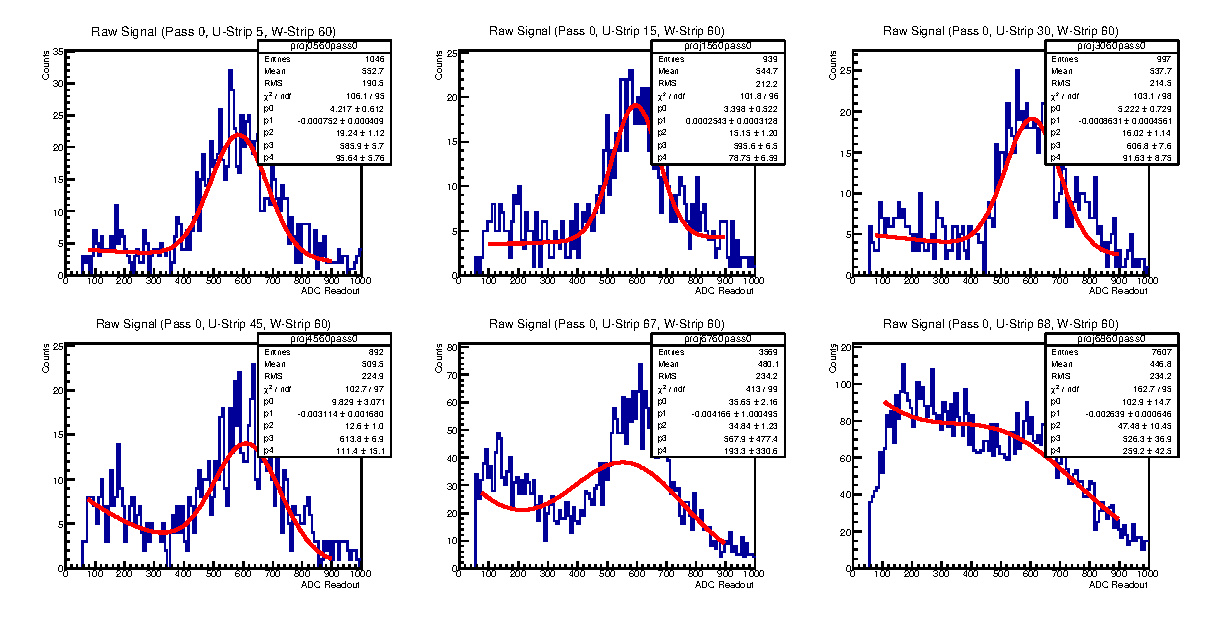
\includegraphics[height= 2.75in, keepaspectratio = true]{pass0}
    \caption{Shown is the ADC signal corresponding to signals from multiple u-strips 
    (5, 15, 30, 45, 67, and 68) and a projection of the w60 strip.}
    \label{fig:pass0}
\end{figure}

\begin{figure}[h]
    \centering
    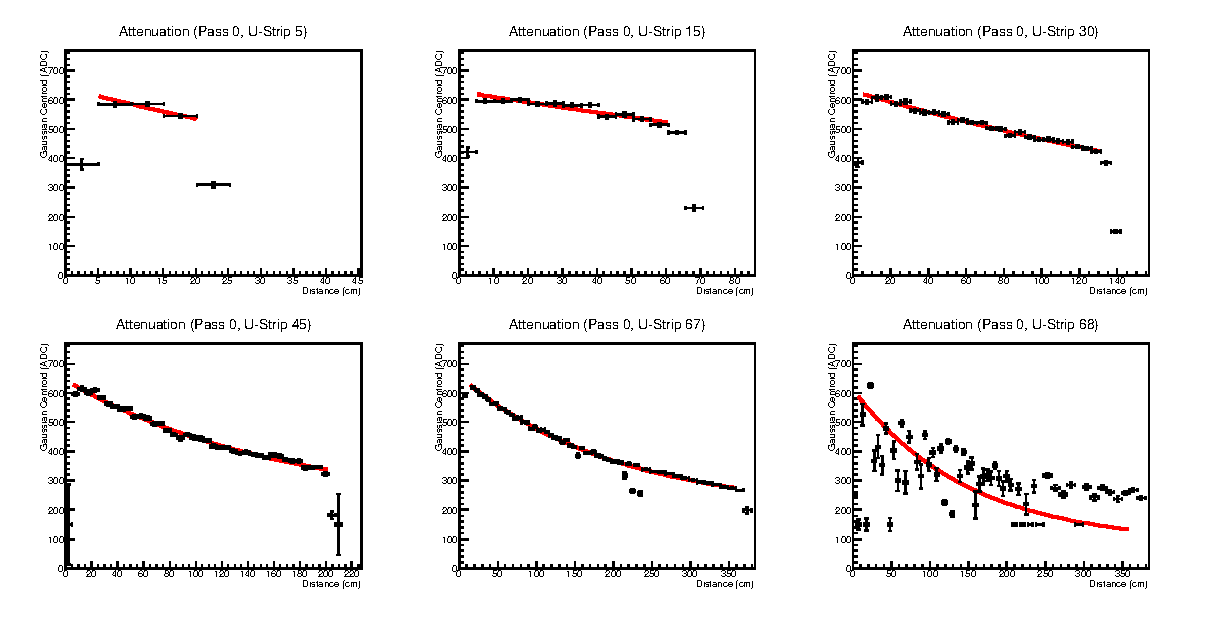
\includegraphics[height= 2.75in, keepaspectratio = true]{atpass0}
    \caption{Shown is the overall attenuation fits to the selected u-strips 
    (5, 15, 30, 45, 67, and 68).}
    \label{fig:atpass0}
\end{figure}


\clearpage
\FloatBarrier
\subsubsection{Pass 1}
\begin{itemize}
    \item Multiplicity Cut: Only events where one PMT fired for each strip were allowed.
    \item Dalitz Cut: An empircal distance sum was used to remove events that don't fall 
    into this range determined by Equation \ref{eq:totaldist}.
    \item Valid hit or near neighbor hit: Using generated events on a calculated skeleton
     of the pcal, each pixel was determined to be valid or not. Extra uncertainty was 
     allowed by also marking nearest neighboring pixels.
    \item 3$\sigma$ Cut on Signal: Each signal was fit to a Gaussian and exponential in 
    pass 0. The parameter $\sigma$ from the Gaussian fit was used to cut out the events
     that did not lie within this function.
\end{itemize}


\begin{figure}[h]
    \centering
    \includegraphics[height= 2.75in, keepaspectratio = true]{pass1}
    \caption{Shown is the ADC signal corresponding to signals from multiple u-strips
     (5, 15, 30, 45, 67, and 68) and a projection of the w60 strip.}
    \label{fig:pass1}
\end{figure}

\begin{figure}[h]
    \centering
    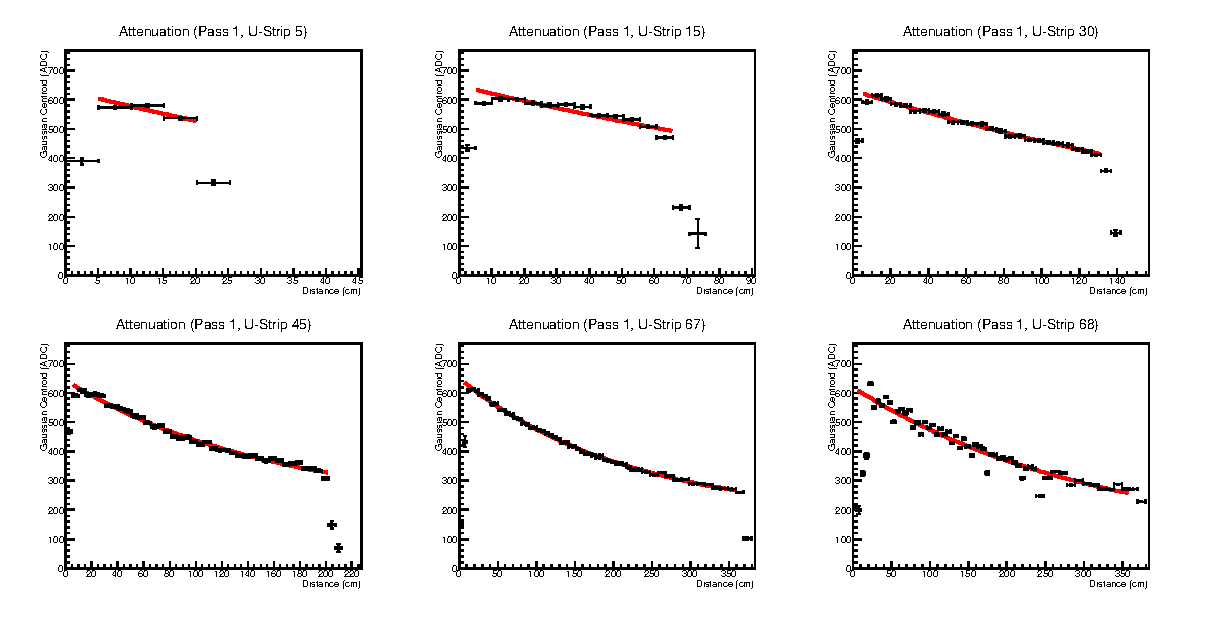
\includegraphics[height= 2.75in, keepaspectratio = true]{atpass1}
    \caption{Shown is the overall attenuation fits to the selected u-strips 
    (5, 15, 30, 45, 67, and 68).}
    \label{fig:atpass1}
\end{figure}



\clearpage
\FloatBarrier
\subsubsection{Pass 2}
\begin{itemize}
    \item Multiplicity Cut: Only events where one PMT fired for each strip were allowed.
    \item Dalitz Cut: An empircal distance sum was used to remove events that don't fall 
    into this range determined by Equation \ref{eq:totaldist}.
    \item Valid hit or near neighbor hit: Using generated events on a calculated skeleton 
    of the pcal, each pixel was determined to be valid or not. Extra uncertainty was allowed 
    by also marking nearest neighboring pixels.
    \item Cut on Attenuation Fits: When the signals where the Gaussian centroid from pass 1 
    were outside an ADC value of $\pm50$ from the attenuation fit, the obtained $\sigma$ was 
    ignored and a new cut about the attenuation fit was employed. If the centroid was close 
    to ADC value from the attenuation fit a 2$\sigma$ cut was used to remove extra background.
\end{itemize}


\begin{figure}[h]
    \centering
    \includegraphics[height= 2.75in, keepaspectratio = true]{pass2}
    \caption{Shown is the ADC signal corresponding to signals from multiple u-strips 
    (5, 15, 30, 45, 67, and 68) and a projection of the w60 strip.}
    \label{fig:pass2}
\end{figure}

\begin{figure}[h]
    \centering
    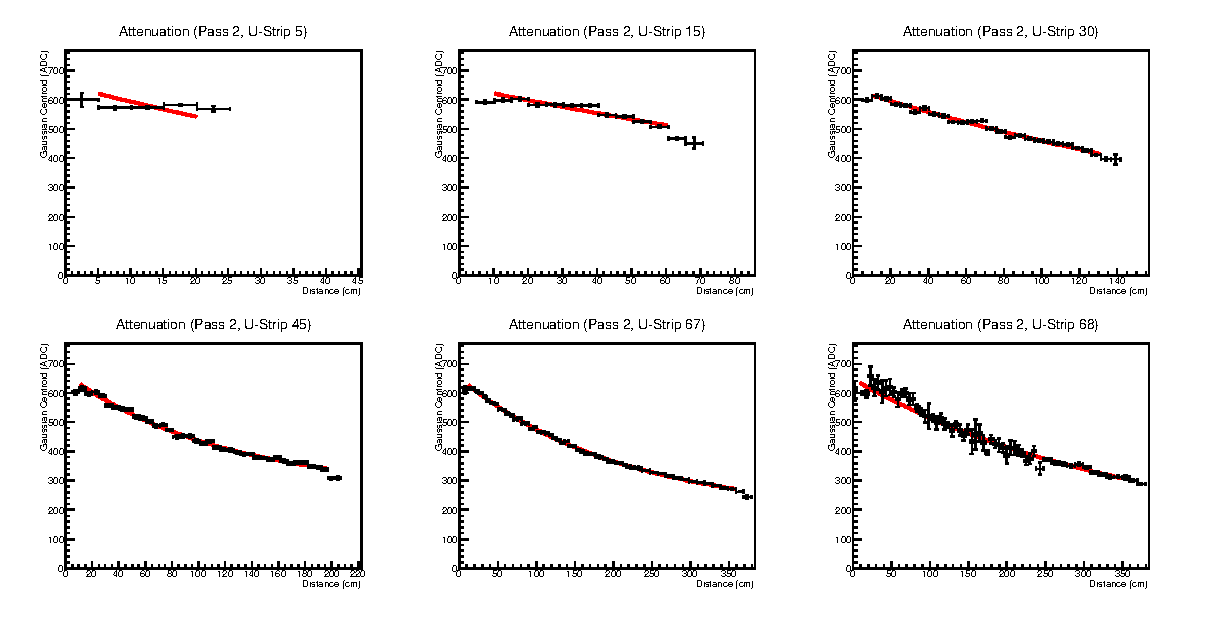
\includegraphics[height= 2.75in, keepaspectratio = true]{atpass2}
    \caption{Shown is the overall attenuation fits to the selected u-strips 
    (5, 15, 30, 45, 67, and 68).}
    \label{fig:atpass2}
\end{figure}



\clearpage
\FloatBarrier
\subsubsection{Pass 3}
\begin{itemize}
    \item Multiplicity Cut: Only events where one PMT fired for each strip were allowed.
    \item Dalitz Cut: An empircal distance sum was used to remove events that don't fall 
    into this range determined by Equation \ref{eq:totaldist}.
    \item Valid hit: Using generated events on a calculated skeleton of the pcal, each 
    pixel was determined to be valid or not.
    \item 3$\sigma$ Cut on Signal: Each signal was fit to a Gaussian in pass 2. The parameter 
    $\sigma$ from the Gaussian fit was used to cut out the events that did not lie within this function.
    \item Attenuation Corrected Intensity Cut: The ADC value measured was corrected with the 
    attenuation curves obtained from pass 2. The corrected value was summed over each layer. 
    A cut on this intensity was placed generously from 1300 to 2700
\end{itemize}

\begin{figure}[h]
    \centering
    \includegraphics[height= 2.75in, keepaspectratio = true]{pass3}
    \caption{Shown is the ADC signal corresponding to signals from multiple u-strips 
    (5, 15, 30, 45, 67, and 68) and a projection of the w60 strip.}
    \label{fig:pass3}
\end{figure}

\begin{figure}[h]
    \centering
    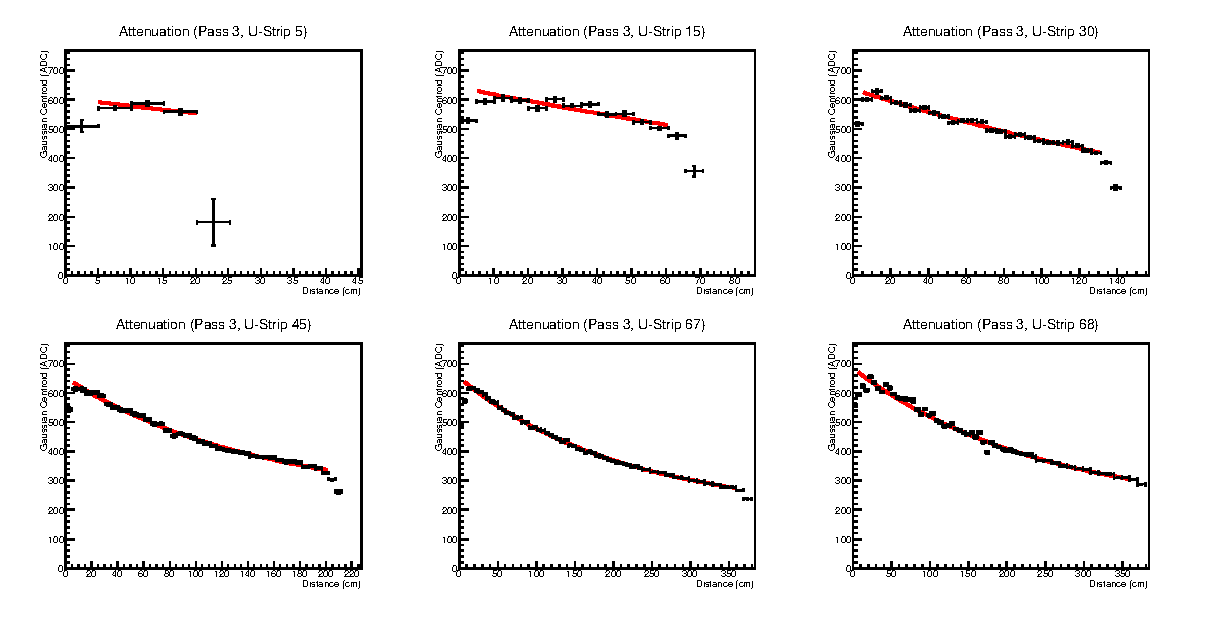
\includegraphics[height= 2.75in, keepaspectratio = true]{atpass3}
    \caption{Shown is the overall attenuation fits to the selected u-strips 
    (5, 15, 30, 45, 67, and 68).}
    \label{fig:atpass3}
\end{figure}

\clearpage
\FloatBarrier
\subsubsection{Pass 4}
\begin{itemize}
    \item Multiplicity Cut: Only events where one PMT fired for each strip were allowed.
    \item Dalitz Cut: An empircal distance sum was used to remove events that don't fall 
    into this range determined by Equation \ref{eq:totaldist}.
    \item Valid hit: Using generated events on a calculated skeleton of the pcal, each 
    pixel was determined to be valid or not.
    \item 3$\sigma$ Cut on Signal: Each signal was fit to a Gaussian in pass 2. The parameter 
    $\sigma$ from the Gaussian fit was used to cut out the events that did not lie within this function.
    \item Attenuation Corrected Intensity Cut: The ADC value measured was corrected with 
    the attenuation curves obtained from pass 2. The corrected value was summed over each 
    layer. A cut on this intensity was placed generously from 1300 to 2700
\end{itemize}


\begin{figure}[h]
    \centering
    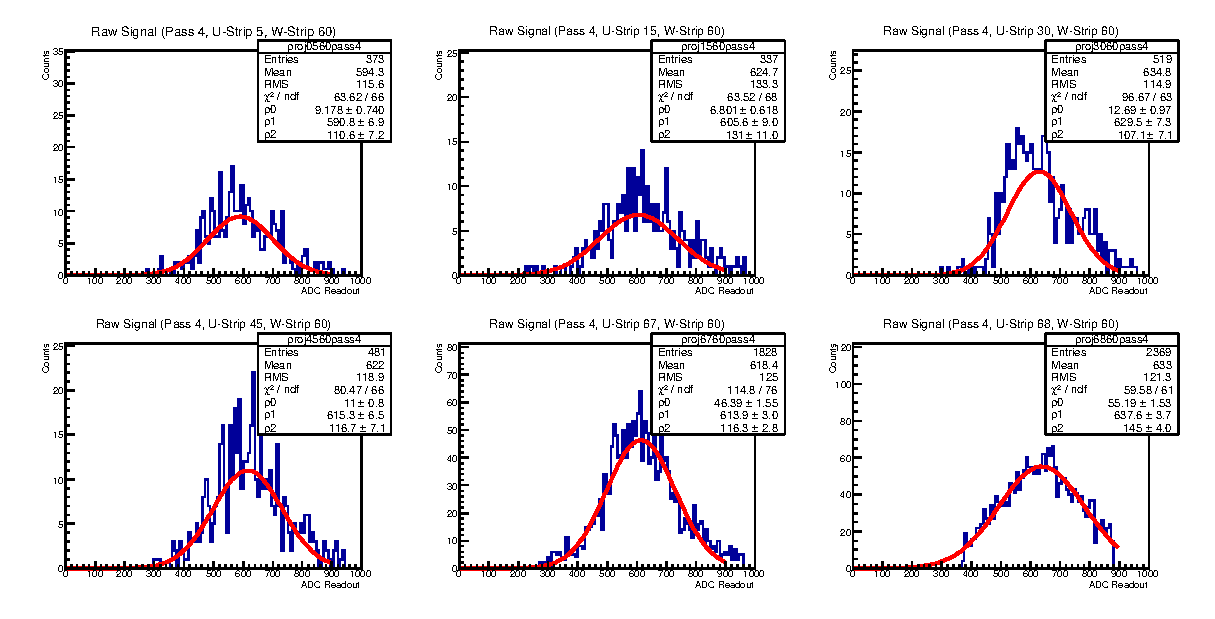
\includegraphics[height= 2.75in, keepaspectratio = true]{pass4}
    \caption{Shown is the ADC signal corresponding to signals from multiple u-strips (5, 15, 30, 45, 67, and 68) and a projection of the w60 strip.}
    \label{fig:pass4}
\end{figure}

\begin{figure}[h]
    \centering
    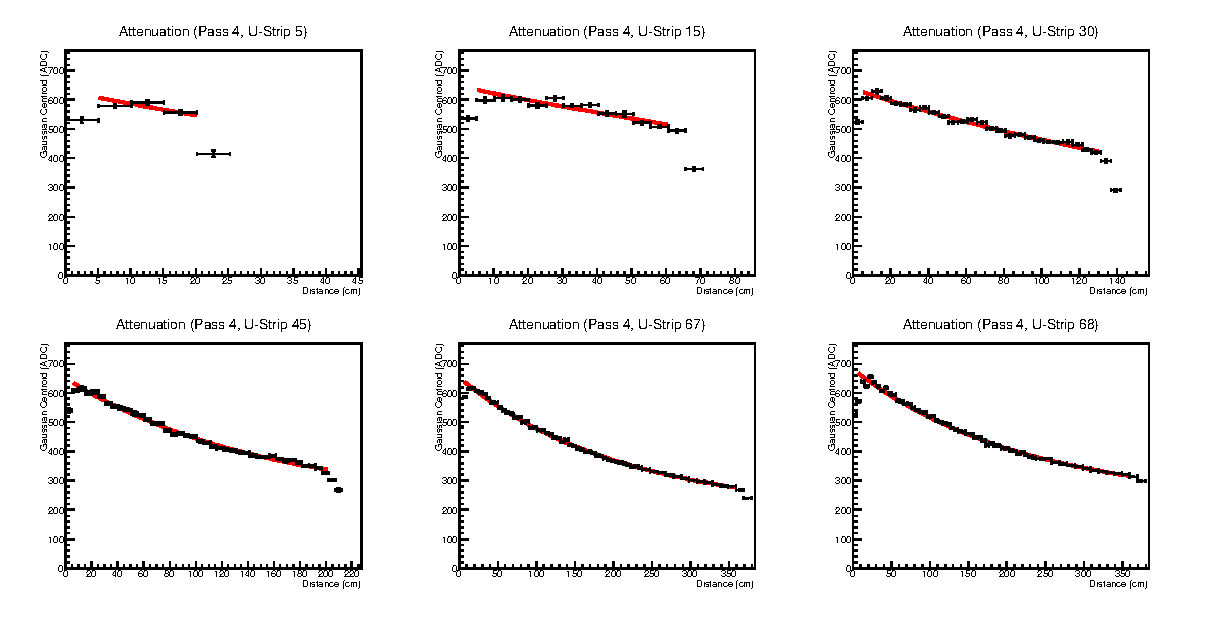
\includegraphics[height= 2.75in, keepaspectratio = true]{atpass4}
    \caption{Shown is the overall attenuation fits to the selected u-strips (5, 15, 30, 45, 67, and 68).}
    \label{fig:atpass4}
\end{figure}


\clearpage
\FloatBarrier
\subsubsection{Pass 5}
\begin{itemize}
    \item Multiplicity Cut: Only events where one PMT fired for each strip were allowed.
    \item Dalitz Cut: An empircal distance sum was used to remove events that don't fall 
    into this range determined by Equation \ref{eq:totaldist}.
    \item Valid hit: Using generated events on a calculated skeleton of the pcal, each pixel 
    was determined to be valid or not.
    \item 3$\sigma$ Cut on Signal: Each signal was fit to a Gaussian in pass 2. The parameter 
    $\sigma$ from the Gaussian fit was used to cut out the events that did not lie within this function.
    \item Attenuation Corrected Intensity Cut: The ADC value measured was corrected with the 
    attenuation curves obtained from pass 2. The corrected value was summed over each layer. 
    A cut on this intensity was placed generously from 1300 to 2700
\end{itemize}
               
               


\begin{figure}[h]
    \centering
    \includegraphics[height= 2.75in, keepaspectratio = true]{pass5}
    \caption{Shown is the ADC signal corresponding to signals from multiple u-strips 
    (5, 15, 30, 45, 67, and 68) and a projection of the w60 strip.}
    \label{fig:pass5}
\end{figure}

\begin{figure}[h]
    \centering
    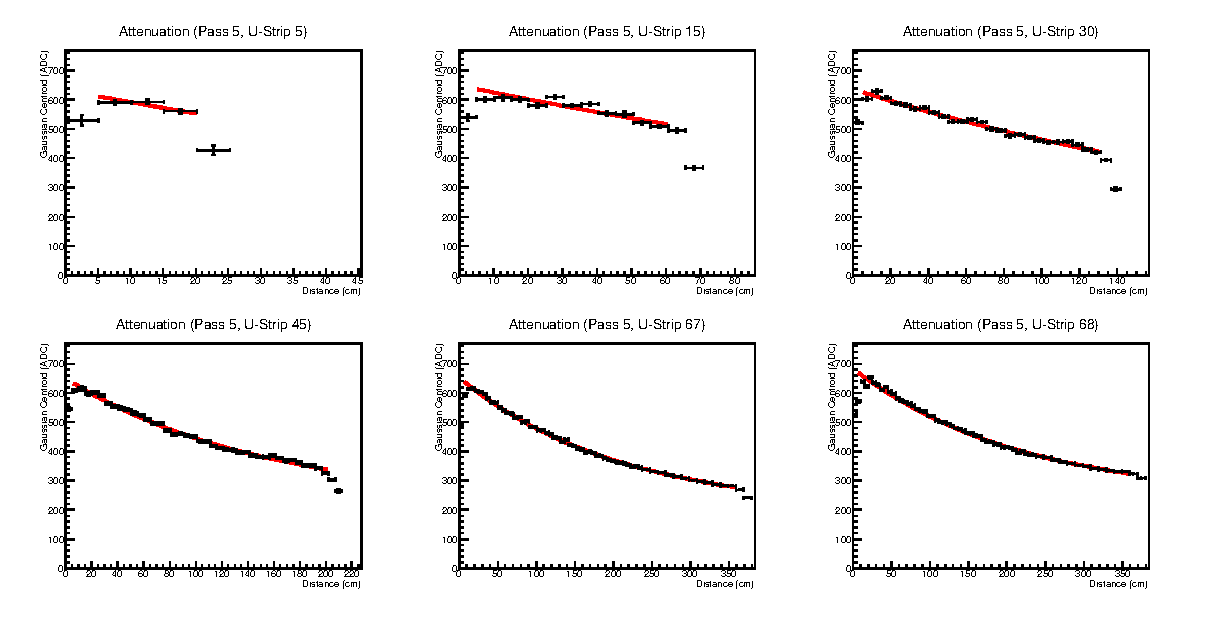
\includegraphics[height= 2.75in, keepaspectratio = true]{atpass5}
    \caption{Shown is the overall attenuation fits to the selected u-strips 
    (5, 15, 30, 45, 67, and 68).}
    \label{fig:atpass5}
\end{figure}


\FloatBarrier


\begin{figure}[h]
    \centering
    \begin{subfigure}[h]{0.3\textwidth}
        \centering
        \includegraphics[width=\textwidth, keepaspectratio = true]{nocutsIsum}
        \caption{Sum of all initial intensities. No cuts.}
        \label{fig:nocutsIsum}
    \end{subfigure}
    ~
    \begin{subfigure}[h]{0.3\textwidth}
        \centering
        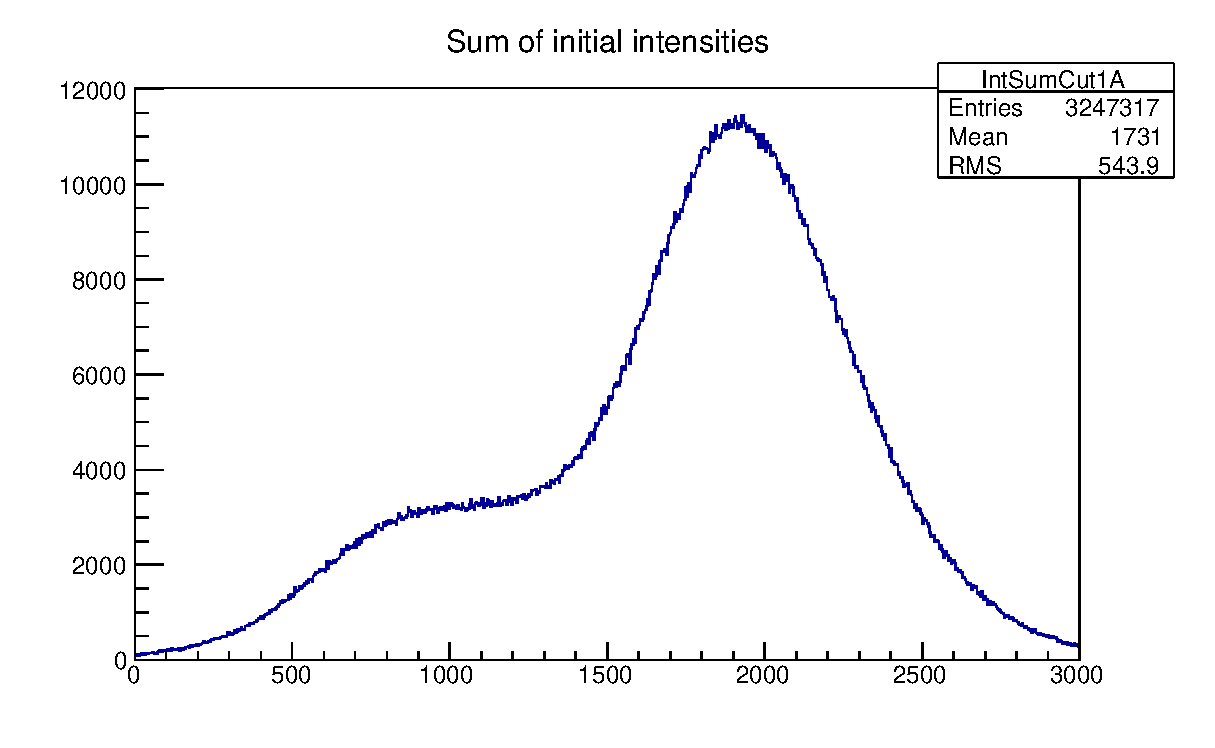
\includegraphics[width=\textwidth, keepaspectratio = true]{3sigcutIsum}
        \caption{Sum of all initial intensities. Three sigma Cut.}
        \label{fig:3sigcutIsum}
    \end{subfigure}
    ~
    \begin{subfigure}[h]{0.3\textwidth}
        \centering
        \includegraphics[width=\textwidth, keepaspectratio = true]{allcutsIsum}
        \caption{Sum of all initial intensities. Three sigma and sum Cut.}
        \label{fig:allcutsIsum}
    \end{subfigure}
    \caption{Sum of initial intensities should be near $650 \times 3 = 1950$ (after gain corrections).}
    \label{fig:intensities}
\end{figure}

\FloatBarrier
\subsection{Comparison of Fits}
Possibly the best evidence for needed cuts about each signal in an iterative process 
is seen by looking at the raw signal fits for a w strip with the possible u projections. 
These comparisons can be seen from pass 0 to pass 5 in Figures \ref{fig:w61sigfitpass0} and 
\ref{fig:w61sigfitpass5}. The difference between these signal tends to be cleaned up to a 
more Gaussian signal. By itself it is difficult to remove the backgound, but due to the correlating 
cuts on the u and v layers a reasonable output is produced.

\begin{figure}[h]
    \centering
    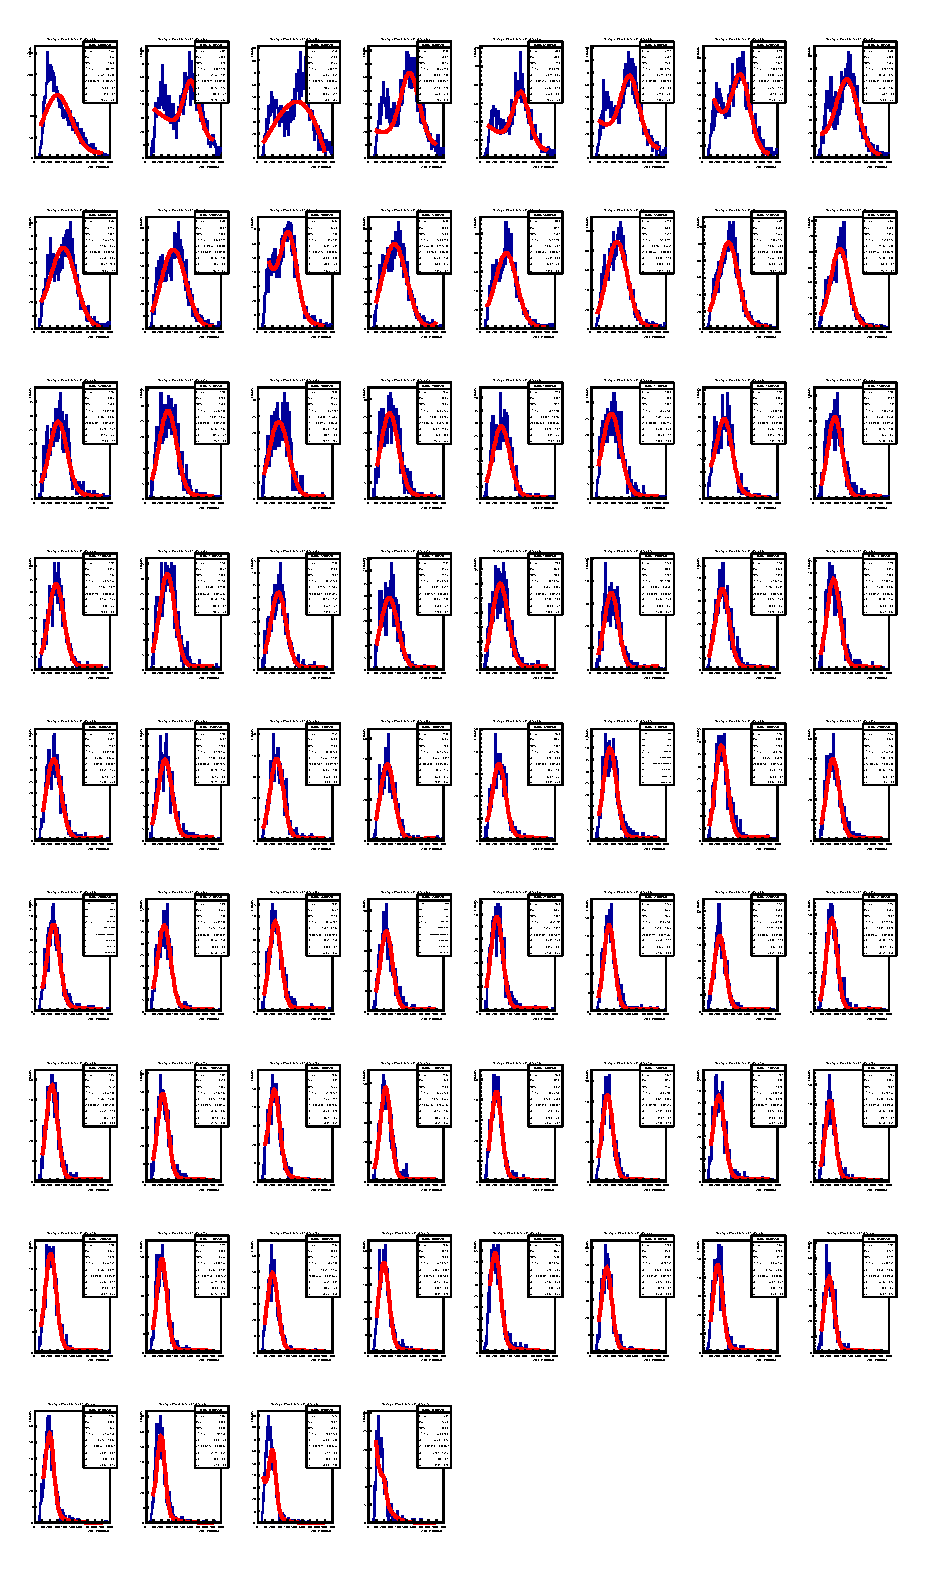
\includegraphics[width=\textwidth, height= 8in, keepaspectratio = true]{w61sigfitpass0}
    \caption{Shown is the ADC signal corresponding to signals from multiple u-strip projections of the w61 strip (pass0).}
    \label{fig:w61sigfitpass0}
\end{figure}

\begin{figure}[h]
    \centering
    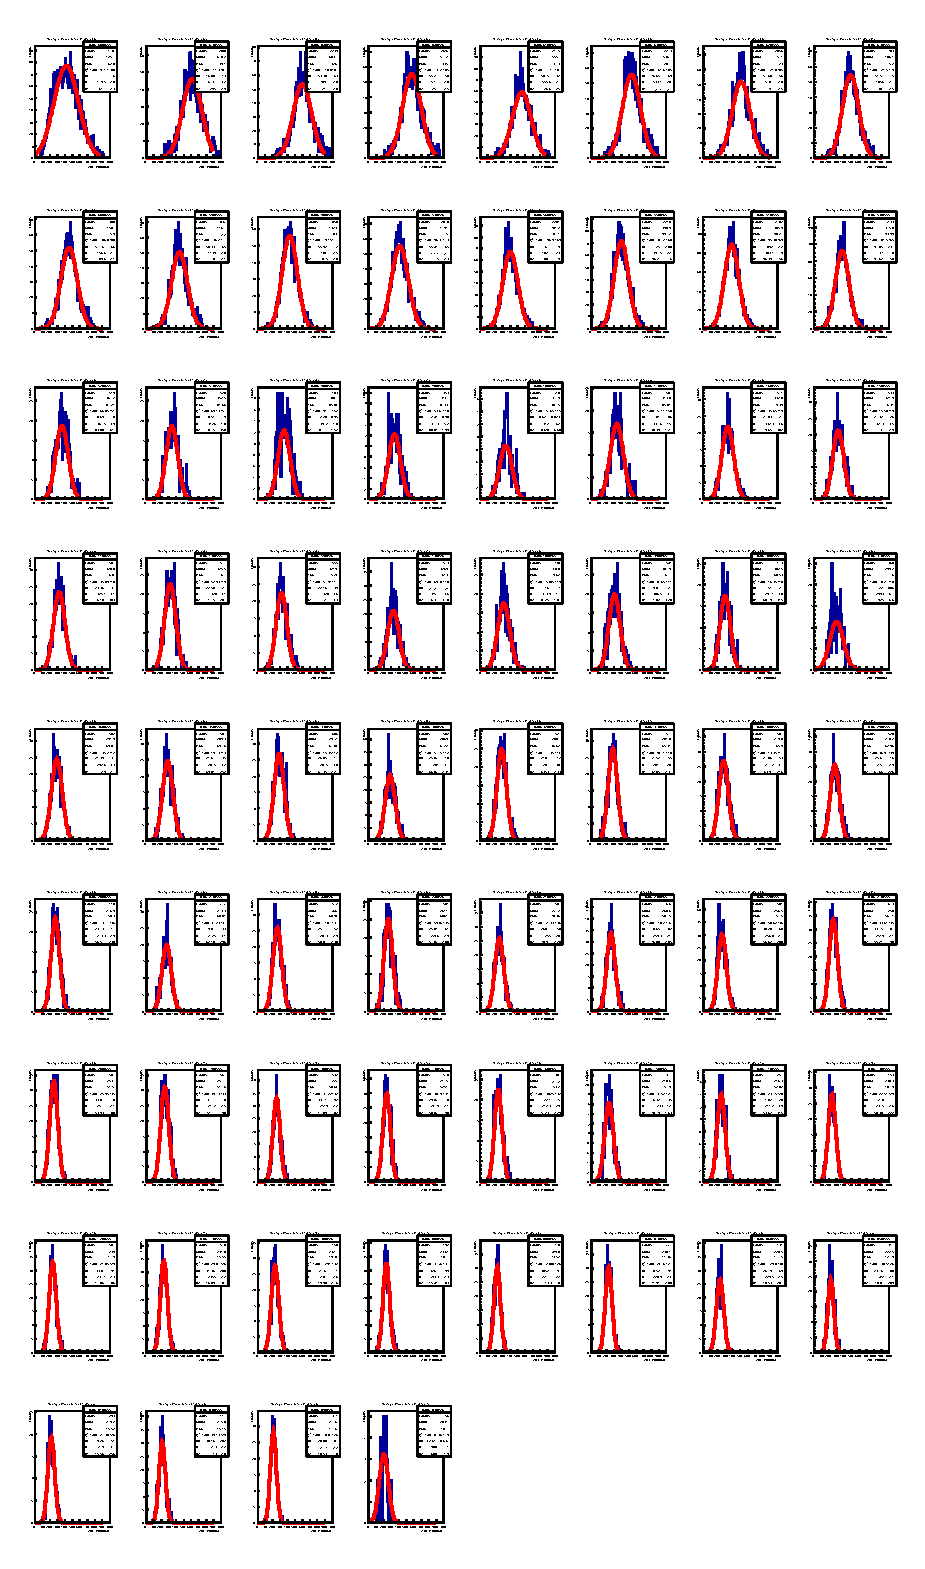
\includegraphics[width=\textwidth, height= 8in, keepaspectratio = true]{w61sigfitpass5}
    \caption{Shown is the ADC signal corresponding to signals from multiple u-strip projections of the w61 strip (pass5).}
    \label{fig:w61sigfitpass5}
\end{figure}


\FloatBarrier

